\usetikzlibrary{calc}
\usetikzlibrary{shapes,arrows}
%% ***********************************************************************
%\textsc{Reinforcement Learning and Dynamic Programming \hfill Spring 2014$\;$ \\
%Lecture Notes \hfill Shie Mannor and Nahum Shimkin \\
%\hfill Scribed by Michal Zarrouk}
%\vspace{-18pt}
%\par
%\hrulefill
%% ***********************************************************************
%
%% {\large
%
%

% \newcommand{\weights}{\texttt{w}}
\newcommand{\ftrs}{\phi}
\newcommand{\FtrMtx}{\Phi}

This chapter starts looking at the case where the MDP model is
large. In the current chapter we will look at approximating the
value function. In the next chapter we will consider learning
directly a policy and optimizing it.

When we talk about a large MDP, it can be due to a few different
reasons. The most common is having a large state space. For example,
Backgammon has over $10^{20}$ states, Go has over $10^{170}$ and robot control typically 
has a continuous state space. The \textit{curse of dimensionality} is a common term for this problem, and relates to states that are composed of several state variables. For example, the configuration of a robot manipulator with $N$ joints can be described using $N$ variables for the angles at each joint. Assuming that each variable can take on $M$ different values, the size of the state space, $M^N$, i.e., grows exponentially with the number of state variables.

Another dimension is the action space,
which can even be continuous in many applications (say, robots).
Finally, we might have complex dynamics which are hard to describe
succinctly (e.g., the next state is the result of a complex simulation), or are not even known to sufficient accuracy. 

Recall Bellman's dynamic programming equation,
$$\Value(\state) = \max_{\action \in \Actions} \left\{\reward(\state,\action) + \gamma \sum_{\state' \in \States} \transitionprob(\state'|\state,\action)\Value(\state')\right\}\quad \forall \state \in \States.$$
Dynamic programming requires knowing the model and is only feasible for small problems, where iterating over all states and actions is feasible. The model-free and model-based learning algorithms described in Chapters \ref{chapter:learning-model-free} and \ref{chapter-model-based} do not require knowing the model, but require storing either value estimates \textit{for each} state and action, or state transition probabilities for every possible state, action, and next state. Scaling up our planning and RL algorithms to very large state and action spaces is the challenge we shall address in this chapter.


\section{Approximation approaches}
There are 4 general approaches to handle the curses of dimensionality:
\begin{enumerate}
\item \textbf{Myopic}: When $\transitionprob(\state'|\state,\action)$ is approximately uniform across $\action$ (i.e., the actions do not affect much the transition to the next state), we may ignore the state transition dynamics and simply use $\policy(\state)\approx \underset{\action \in \Actions}{\operatorname{argmax}} \{\reward(\state,\action)\}$. If $\reward(\state,\action)$ is not known exactly -- replace it with an estimate.

\item \textbf{Lookahead policies}: Rolling horizon/model-predictive control.\\
At each step $\ttime$, simulate a horizon of $\tHorizon$ steps, and use
$$\policy(\state_\ttime) = \underset{\policy' \in \Policies}{\operatorname{argmax}}\  \mathbb{E}^{\policy'} \left[\left.\sum_{\ttime'=\ttime}^{\ttime+\tHorizon} \reward(\state_{\ttime'},\action_{\ttime'})\right|\state_\ttime\right].$$

\item \textbf{Policy function approximation}\\
Assume the policy is of some parametric function form $\policy = \policy(\weight), \ \ \weight \in \mathtt{W}$, and optimize over function parameters.\\
% \begin{example}[Inventory management]
% Consider an inventory management problem, in which the state is the inventory level $\state_\ttime$, the demand is $d_\ttime$ and the action is the replenishment level $\action_\ttime$. The dynamics are given by:
% $$s_{t+1} = [\state_\ttime + \action_\ttime-d_\ttime]^+.$$
% The immediate reward is:
% $$R_\ttime = R \min\{d_\ttime,\state_\ttime+\action_\ttime\} - c_a \action_\ttime -C[\state_\ttime + \action_\ttime-d_\ttime]^+,$$
% where $R$ is the profit in satisfying the demand, $c_a$ is the ordering cost, and $C$ is the cost of not satisfying a demand.

% One possible replenishment policy is:
% $$a^\pi(\state_\ttime|\weights) = \begin{cases} 0 & \state_\ttime > q\\Q-\state_\ttime & \state_\ttime \le q \end{cases}, \ \ \ \weights=(q,Q).$$
% A different possibility is the \emph{softmax} policy, given by
% $$p(s,a) = \frac{e^{-\weights\alpha(s,a)}}{\sum_{a'} e^{-\weights\alpha(s,a')}}, \ \ \mathrm{where}\ \ \alpha=R(s,a)\ \ \mathrm{or} \ \ \alpha=Q(s,a).$$
% \end{example}

\item \textbf{Value function approximation}\\
In problems where computing the value function directly is intractable, due to the reasons described above, we consider an approximate value function of some parametric form.
When considering a value function approximation, there are a few interpretations
to what exactly we mean. Given a policy $\policy$, it can either be: (1) mapping from a state
$\state$ to its expected return, i.e.,
$\widehat{\Value}^\policy(\state;\weight)$. (2) mapping from state-action
pairs $(\state,\action)$ to their expected return, i.e.,
$\widehat{Q}^\policy(\state,\action;\weight)$. (3) mapping from
states $\state$ to expected return of each action, i.e.,
$\{\widehat{Q}^\policy(\state,\action_i;\weight):\action_i\in
\Actions\}$. All the interpretations are valid, and our
discussion will not distinguish between them (actually, for
$\{\widehat{Q}^\policy(\state,\action_i;\weight):\action_i\in
\Actions\}$ we implicitly assume that the number of actions is
small). We shall also be interested in approximating the optimal value function, and the corresponding approximations are denoted $\widehat{\Value}^*(\state;\weight)$, $\widehat{Q}^*(\state,\action;\weight)$, and $\{\widehat{Q}^*(\state,\action_i;\weight):\action_i\in
\Actions\}$, respectively.\\
Given an approximate $\widehat{Q}^*(\state,\action;\weight)$, we can derive an approximately optimal policy by choosing the \emph{greedy} action with respect to $\widehat{Q}^*(\state,\action;\weight)$.
\end{enumerate}

We mention that the approaches above are not mutually exclusive, and often in practice, the best performance is obtained by combining different approaches. For example, a common approach is to combine a $\tHorizon$ step lookahead with an approximate terminal value function, 
\begin{equation*}
    \policy(\state_\ttime) = \underset{\pi' \in \Pi}{\operatorname{argmax}}\  \mathbb{E}^{\policy'} \left[\sum_{\ttime'=\ttime}^{\ttime+\tHorizon-1} \reward(\state_{\ttime'}) + \widehat{\Value}^*(\state_{\ttime+\tHorizon}))\right].
\end{equation*}
We shall also see, in the next chapter, that value function approximations will be a useful component in approximate policy optimization. In the rest of this chapter, we focus on value function approximation. 
We will consider (mainly) the discounted return with
a discount parameter $\gamma\in(0,1)$. The results extend very
naturally to the finite horizon and episodic settings.

% \tikzstyle{block} = [rectangle, draw,
%     text width=7em, text centered, rounded corners, minimum height=4em]
% \tikzstyle{blocks} = [rectangle, draw,
%     text width=4em, text centered, rounded corners, minimum height=4em]
% \tikzstyle{lblock} = [rectangle, draw,
%     text width=17em, text centered, rounded corners, minimum height=4em]
% \tikzstyle{line} = [draw, -latex']
% \begin{tikzpicture}[node distance = 1cm, auto]
%     % Place nodes
% %    \node [blocks] (a) {Chess game model};
%     \node [block] (b) {Feature extraction\\$\ftrs_1(s),...,\ftrs_k(s)$};
%     \node [block, right of = b, node distance=1.3in] (c) {Compute value\\function weights\\$\weight_1,...,\weight_k$};
%     \node [block, right of = c, node distance=1.3in] (d) {Set\\ $\widehat{\Value}^*(\state;\weight)$};
%     \node [lblock, right of = d, node distance=2.1in] (e) {\small$\policy(\state_\ttime) = \underset{\pi' \in \Pi}{\operatorname{argmax}}\  \mathbb{E}^{\policy'} \left[\sum_{\ttime'=\ttime}^{\ttime+\tHorizon-1} \reward(\state_{\ttime'}) + \widehat{\Value}^*(\state_{\ttime+\tHorizon}))\right]$};
%     % Draw edges
% %    \path [line] (a) -- (b);
%     \path [line] (b) -- (c);
%     \path [line] (c) -- (d);
%     \path [line] (d) -- (e);
% \end{tikzpicture}

\subsection{Value Function Approximation Architectures}

We now need to discuss how will we build the approximating function.
For this we can turn to the rich literature in Machine Learning and
consider popular hypothesis classes. For example: (1) Linear
functions, (2) Neural networks, (3) Decision trees, (4) Nearest
neighbors, (5) Fourier or wavelet basis, etc. We will concentrate
here on linear functions.
% and neural networks, mainly since gradient based methods apply to them very naturally.

In a linear function approximation, we represent the value as a weighted combination of some $\nftrs$ features:
$$\widehat{\Value}^\policy(\state;\weight) = \sum_{j=1}^\nftrs \weight_j \ftrs_j(\state) = \weight^T \ftrs(\state),$$
where $\weight \in \mathbb{R}^\nftrs$ are the model parameters and $\ftrs(\state) \in \mathbb{R}^\nftrs$ are the model's \emph{features} (a.k.a. basis functions). Similarly, for state-action value functions, we use state-action features, $\ftrs(\state,\action)\in \mathbb{R}^\nftrs$, and approximate the value by $\widehat{Q}^\policy(\state,\action;\weight) =  \weight^T \ftrs(\state,\action)$.

Popular example of state feature vectors include radial basis functions $\phi_j(\state) \propto \exp(\frac{(\state-\mu_j)^2}{\sigma_j})$, and tile features, where $\phi_j(\state) = 1$ for a set of states $A_j \subset \States$, and $\phi_j(\state) = 0$ otherwise. For state-action features, when the number of actions is finite $\Actions = \left\{1,2,\dots,|\Actions|\right\}$, a common approach is to extend the state features independently for every action. That is, consider the following construction for $\ftrs(\state,i)\in \mathbb{R}^{\nftrs \cdot |\Actions|}$, $i\in \Actions$:
\begin{equation*}
    \ftrs(\state,i)^T = \left[ \underbrace{\mathbf{0}^T, \mathbf{0}^T, \dots, \mathbf{0}^T}_{i-1 \text{ times}}, \ftrs(\state)^T, \underbrace{\mathbf{0}^T, \dots, \mathbf{0}^T}_{|\Actions|-i \text{ times}}\right],
\end{equation*}
where $\mathbf{0}$ is a vector of $\nftrs$ zeros.

For most interesting problems, however, designing appropriate features is a difficult problem that requires significant domain knowledge, as the structure of the value function may be intricate. In the following, we assume that the features $\ftrs(\state)$ (or $\ftrs(\state,\action)$) are given to us in advance, and we will concentrate on general methods for calculating the weights $\weight$ in a way that minimizes the approximation error as best as possible, with respect to the available features. 

\section{Quantification of Approximation Error}

Before we start the discussion on the learning methods, we will do a
small detour. We will discuss the effect of having an error in the
value function we learn, and its effect on the outcome. Assume we
have a value function $\widehat{\Value}$ such that $\|\widehat{\Value}-\Value^*\|_\infty\leq
\varepsilon$. Let $\widehat{\policy}$ be the greedy policy with respect to
$\widehat{\Value}$, namely,
\[
\widehat{\policy}(\state)=\arg\max_\action [\reward(\state,\action)+\gamma
\mathbb{E}_{\state'\sim \transitionprob(\cdot|\state,\action)}[\widehat{\Value}(\state')].
\]


\begin{theorem}\label{thm:approx_error}
Let $\widehat{\Value}$ such that $\|\widehat{\Value}-\Value^*\|_\infty\leq \varepsilon$ and
$\widehat{\policy}$ be the greedy policy with respect to $\widehat{\Value}$. Then,
\[
\|\Value^{\widehat{\policy}}-\Value^*\|_\infty\leq\frac{2\gamma\varepsilon}{1-\gamma}.
\]
\end{theorem}

\begin{proof}
Consider two operators $\operator^\policy$ and $\operator^*$ (see
Chapter \ref{ss:DP_op}). The first, $\operator^\policy$, is
\[
(\operator^\policy v)(\state)=\reward(\state,\policy(\state))+\gamma
\mathbb{E}_{\state'\sim \transitionprob(\cdot|\state,\policy(\state))}[v(\state')],
\]
and it converges to $\Value^\policy$ (see Theorem~\ref{thm:DP_op}).
The second, $\operator^*$, is
\[
(\operator^* v)(\state)=\max_\action[\reward(\state,\action)+\gamma
\mathbb{E}_{\state'\sim \transitionprob(\cdot|\state,\action)}[v(\state')] ],
\]
and it converges to $\Value^*$ (see Theorem~\ref{thm:DP_op}).
In addition, recall that we have shown that both
$\operator^\policy$ and $\operator^*$ are $\gamma$-contracting (see
Theorem~\ref{thm:DP_op}).

Since $\widehat{\policy}$ is greedy with respect to $\widehat{\Value}$ we have
$\operator^{\widehat{\policy}} \widehat{\Value}=\operator^* \widehat{\Value}$ (but this does not hold for
other value functions $\Value' \neq \widehat{\Value}$).

Then,
\begin{align*}
\|\Value^{\widehat{\policy}}-\Value^*\|_\infty &= \|\operator^{\widehat{\policy}} \Value^{\widehat{\policy}} - \Value^*\|_\infty\\
&\leq \|\operator^{\widehat{\policy}} \Value^{\widehat{\policy}} -\operator^{\widehat{\policy}} \widehat{\Value}\|_\infty +\|\operator^{\widehat{\policy}} \widehat{\Value} - \Value^*\|_\infty\\
&\leq \gamma\| \Value^{\widehat{\policy}} - \widehat{\Value}\|_\infty +\|\operator^* \widehat{\Value} - \operator^*\Value^*\|_\infty\\
&\leq \gamma\| \Value^{\widehat{\policy}} - \widehat{\Value}\|_\infty +\gamma\| \widehat{\Value} - \Value^*\|_\infty\\
&\leq \gamma(\| \Value^{\widehat{\policy}} - \Value^*\|_\infty+ \|\Value^*-\widehat{\Value}\|_\infty ) +\gamma\| \widehat{\Value} - \Value^*\|_\infty\;,
\end{align*}
where in the second inequality we used the fact that since since
$\policy$ is greedy with respect to $\widehat{\Value}$ then $\operator^{\widehat{\policy}} \widehat{\Value}=\operator^* \widehat{\Value}$.

Reorganizing the inequality and recalling that
$\|\Value^*-\widehat{\Value}\|_\infty\leq \varepsilon$, we have
\[
(1-\gamma)\|\Value^{\widehat{\policy}}-\Value^*\|_\infty \leq 2\varepsilon\gamma,
\]
and the theorem follows.
\end{proof}

The above theorem states that if we have small errors in
$L_\infty$ norm, the effect of the errors on the expected return is
bounded. However, in most cases we will not be able to guarantee an
approximation in norm $L_\infty$. This is since it is infeasible even
to compute the $L_\infty$ norm of two given value functions, as the computation requires considering {\em all} states. In the large state space setting, such operations are infeasible. 

Intuitively, a more feasible guarantee is that some \textit{average} error is small. In the following, we shall see that this condition can be represented mathematically as a weighted $L_2$ norm. Extending Theorem \ref{thm:approx_error} to a weighted $L_2$ norm is possible, but is technically involved~\cite{munos2007performance}, and we will not consider it in this book. Nevertheless, we shall next study learning algorithms that have a guaranteed average error bound.

\section{From RL to Supervised Learning}

To learn the value function, we would like to reduce our reinforcement learning problem to a
supervised learning problem. This will enable us to use any of the many techniques of machine learning to address the problem. Let us consider the basic ingredients of supervised learning. The most important ingredient is having a labeled sample set, which is sampled i.i.d.

Let us start by considering an idealized setting. Fix a policy $\policy$, and consider learning its value function $\widehat{\Value}^{\policy}$. To apply supervised learning, we should
generate a training set, i.e., 
\[
\{(\state_1, \Value^\policy(\state_1)),\ldots,
(\state_m,\Value^\policy(\state_m))\}.
\]
We first need to discuss how to sample the states $\state_i$ in an
i.i.d. way. We can generate trajectory, but we need to be careful,
since adjacent states are definitely dependent! One solution is to
space the sampling from the trajectory using the mixing time of
$\policy$.\footnote{See Chapter \ref{chapter:MC} for definition.}
This will give us samples $\state_i$ which are sampled (almost) from the
stationary distribution of $\policy$ and are (almost) independent. In the episodic setting, we can sample different episodes, and states from different episodes are guaranteed to be independent.
%For the action, we clearly will use $\policy$, no problem there.

Second, we need to define a loss function, which will tradeoff the different approximation errors. Since the value is a real scalar, a natural candidate is the average squared error loss, $\frac{1}{m}\sum_{i=1}^m (\widehat{\Value}^\policy(\state_i) - \Value^\policy(\state_i))^2$. With this loss, the corresponding supervised learning problem is least squares regression.

The hardest, and most confusing, ingredient is the labels
$\Value^\policy(\state_i)$. In supervised machine leaning we assume
that someone gives us the labels to build a classifier.
% (or alternatively, in unsupervised learning, where there is no clear ground truth).
However, in our problem, the value function is exactly what we want to learn, and it is not realistic to assume any ground truth samples from it!

Our main task, therefore, would be to replace the ground truth labels with quantities that we can measure, using simulation or interaction with the system. We shall start by formally defining least squares regression in a way that will be convenient to extend later to RL.



% \section{Approximation Methods in Value Space}
% \begin{enumerate}
% \item Approximate policy iteration: approximate $\Value^\policy$; improve $\policy$; repeat.
% \item Approximate value iteration / Q-learning: $\widehat{Q}(s,a)\approx {\ftrs}(s,a)^\top {\weight}$
% % \item Bellman error minimization:
% % $$ \min_\weights \  \mathbb{E}_s \left[\left(\tilde{V}(s;\weights)-T\tilde{V}(s;\weights)\right)^2\right]$$
% % where $T$ is the Bellman operator and $\mathbb{E}_s$ is w.r.t. some distribution over the states.
% \item Linear programming: not discussed.
% \end{enumerate}

% Note that both $V$ and $Q$ are mappings from a state (or state-action) to $\mathbb{R}$. When the state space is large, we will not be able to calculate the value for every state, but instead, fit an approximate function based on a few states for which their values can be calculated (or estimated). This is similar to a \emph{regression} problem, which our development will be based on, but as we shall see, we will also need to account for the dynamic nature of the problem to develop approximate optimization algorithms.

% \subsection{Approximate Policy Evaluation}

% We start with the simplest setting - approximating the value of a fixed policy. A direct approach for this task is through regression, which we will now review. 

\subsection{Preliminaries -- Least Squares Regression}
To simplify our formulation, we will assume that the state space may be very large, but finite. Equivalently, we will consider a regression problem where the independent variable can only take a finite set of values. 

Assume we have some function $y = f(x)$, where $y \in \mathbb{R}$, $x\in X$, and $X$ is finite. As in standard regression analysis, $x$ is termed the independent variable, while $y$ is the dependent variable. We assume that data is generated by sampling i.i.d. from a distribution $\xi(x)$, and the labels are noisy. That is, we are given $N$ labeled samples $\left\{(x_1, y_1),\dots, (x_N, y_N) \right\}$, where $x_i \sim \xi(x)$, $y_i = f(x_i) + \omega(x_i)$, and $\omega(x)$ is a zero-mean i.i.d. noise (which may depend on the state).

Our goal is to fit to our data a parametric function $g(x;\weights):X \to \mathbb{R}$, where $\weights \in \mathbb{R}^{\nftrs}$, such that $g$ approximates $f$ well. The Least Squares approach solves the following problem:
\begin{equation}\label{eq:least_squares}
\hat{\weights}_{LS} = \min_\weights \frac{1}{N}\sum_{i=1}^N (g(x_i;\weights) - y_i)^2.
\end{equation}
A practical iterative algorithm for solving \eqref{eq:least_squares} is the stochastic gradient descent (SGD) method, which updates the parameters by
\begin{equation}\label{eq:sgd}
\weights_{i+1} = \weights_i - \alpha_i (g(x_i;\weights_i) - y_i)\nabla_\weights g(x_i;\weights_i),
\end{equation}
where $\alpha_i$ is some step size schedule, such as $\alpha_i = 1/i$.
% $$
% \min_\weights \mathbb{E}_{x\sim\xi} (g(x;\weights) - f(x))^2.
% $$



When $g$ is linear in some features $\ftrs(x)$, i.e., $g(x;\weights) = \weights^T \ftrs(x)$, the least squares solution can be calculated explicitly. Let $\hat{\FtrMtx} \in \mathbb{R}^{N \times \nftrs}$ be a matrix with $\ftrs(x_i)$ in its rows, often called the \textit{design matrix}. Similarly, let $\hat{Y}\in \mathbb{R}^{N \times 1}$ be a vector of $y_i$'s. Then, Equation \eqref{eq:least_squares} can be written as
\begin{equation}\label{eq:linear_least_squares}
\hat{\weights}_{LS} = \min_\weights \frac{1}{N} (\hat{\FtrMtx} \weights - \hat{Y})^T(\hat{\FtrMtx} \weights - \hat{Y}) = 
\min_\weights \frac{1}{N} \left( \weights^T (\hat{\FtrMtx}^T \hat{\FtrMtx}) \weights -2 \weights^T \hat{\FtrMtx}^T \hat{Y} + \hat{Y}^T\hat{Y} \right).
\end{equation}
Noting that \eqref{eq:linear_least_squares} is a quadratic form, the least squares solution is calculated to be: 
\begin{equation}\label{eq:sampled_LS}
    \hat{\weights}_{LS} = (\hat{\FtrMtx}^T \hat{\FtrMtx})^{-1} \hat{\FtrMtx}^T \hat{Y}.
\end{equation}

We now characterize the LS solution when $N \to \infty$, which  will allow us to talk about the \textit{expected} least squares solution. Without loss of generality, we assume that the states are ordered, $1,2,\dots,|X|$. Let $\xi\in \mathbb{R}^{|X|}$ denote a vector with elements $\xi(x)$, and define the diagonal matrix
$\Xi = \text{diag}(\xi)\in\mathbb{R}^{|X| \times |X|}$. Further, let $\FtrMtx \in \mathbb{R}^{|X| \times \nftrs}$ be a matrix with $\ftrs(x)$ as its rows, and let $Y\in \mathbb{R}^{|X|}$ be a vector of $f(x)$.


\begin{proposition}
Assume that $\FtrMtx^T \Xi \FtrMtx$ is not singular. We have that $\lim_{N \to \infty} \hat{\weights}_{LS} = \weights_{LS}$, where
\begin{equation*}
    \weights_{LS} = (\FtrMtx^T \Xi \FtrMtx)^{-1} \FtrMtx^T \Xi Y.
\end{equation*}
\end{proposition}

\begin{proof}
From the law of large numbers, we have that 
\begin{equation*}
\begin{split}
    \lim_{N \to \infty}\frac{1}{N}\hat{\FtrMtx}^T \hat{\FtrMtx} &= \lim_{N \to \infty}\frac{1}{N} \sum_{i=1}^N \phi(x_i) \phi(x_i)^T \\
    &= \mathbb{E}_{x \sim \xi(x)}\left[ \phi(x) \phi(x)^T \right] \\
    &= \sum_{x} \xi(x) \phi(x) \phi(x)^T \\
    &= \FtrMtx^T \Xi \FtrMtx.
\end{split}
\end{equation*}
Similarly, $\lim_{N \to \infty}\frac{1}{N} \hat{\FtrMtx}^T \hat{Y} = \FtrMtx^T \Xi Y$. Plugging into Eq.~\eqref{eq:sampled_LS} completes the proof.
\end{proof}

Using the stochastic approximation technique, a similar result holds for the SGD update.
\begin{proposition}
Consider the SGD update in Eq.~\eqref{eq:sgd} with linear features, 
$$
\weights_{i+1} = \weights_i - \alpha_i ( \weights^T \ftrs(x_i) - y_i)\ftrs(x_i).
$$
Assume that $\FtrMtx^T \Xi \FtrMtx$ is not singular, and that the step sizes satisfy $\sum_i \alpha_i = \infty$ and $\sum_i \alpha_i^2 < \infty$. Then $\weights_{i} \to \weights_{LS}$ almost surely. 
\end{proposition}

Note that the expected LS solution can also be written as the solution to the following \textit{expected least squares} problem:
\begin{equation}\label{eq:LS_expected}
\weights_{LS} = \min_\weights (\FtrMtx \weights - Y)^T \Xi (\FtrMtx \weights - Y).
\end{equation}
Observe that $\FtrMtx \weights_{LS} \in \mathbb{R}^{|X|}$ denotes a vector that contains the approximated function $g(x;\weights_{LS})$ for every $x$. This is the best approximation, in terms of expected least square error, of $f$ onto the linear space spanned by the features $\ftrs(x)$. Recalling that $Y$ is a vector of ground truth $f$ values, we view this approximation as a \emph{projection} of $Y$ onto the space spanned by $\FtrMtx \weights$, and we can write the projection operator explicitly as:
$$
\Project_\xi Y = \FtrMtx \weights_{LS} = \FtrMtx (\FtrMtx^T \Xi \FtrMtx)^{-1} \FtrMtx^T \Xi Y.
$$

Geometrically, $\Project_\xi Y$ is the vector that is closest to $Y$ on the linear subspace $\FtrMtx \weights$, where the distance function is the $\xi$-weighted Euclidean norm, $||z||_\xi = \sqrt{\langle z,z\rangle_\xi}$, where $\left\langle z, z' \right \rangle_\xi = z^T \Xi z'$.

We conclude this discussion by noting that although we derived Eq.~\eqref{eq:LS_expected} as the expectation of the least square method, we could also take an alternative view: the least squares method in \eqref{eq:sampled_LS} and the SGD algorithm are two different \textit{sampling} based approximations to the expected least squares solution in \eqref{eq:LS_expected}. We will take this view when we develop our RL algorithms later on.

% In the non-linear case, a common approach is to solve the least squares problem by gradient descent, i.e., $\weights_{k+1} = \weights_k - \alpha_k \nabla_\weights \mathbb{E}_{x\sim\xi} (g(x;\weights) - f(x))^2,$ where the gradient is simply $2 \mathbb{E}_{x\sim\xi} (g(x;\weights) - f(x))\nabla_\weights g(x;\weights)$. 

% In a practical case, we are given $N$ data samples $\{ x_i, y_i \}: x_i\sim \xi, y_i=f(x_i)$. The least squares solution can be approximated from the samples as:
% $$
% \min_\weights \sum_i (g(x_i;\weights) - y_i)^2,
% $$
% The stochastic gradient descent (SGD) version of this update is
% $$
% \weights_{k+1} = \weights_k - \alpha_k (g(x_i;\weights_k) - y_i)\nabla_\weights g(x_i;\weights_k).
% $$

% For the linear case, we can solve directly:
% $$
% \hat{\weights}_{LS} = (\hat{\FtrMtx}^T \hat{\FtrMtx})^{-1} \hat{\FtrMtx}^T \hat{Y},
% $$
% where in this case the rows of $\hat{\FtrMtx}$ and $\hat{Y}$ are given by the $N$ samples. By the law of large numbers, we have that $\frac{1}{N}(\hat{\FtrMtx}^T \hat{\FtrMtx}) \to (\FtrMtx^T \Xi \FtrMtx)$ and $\frac{1}{N}\hat{\FtrMtx}^T \hat{Y} \to \FtrMtx^T \Xi Y$, thus the sampled solution converges to the solution $\weights_{LS}$ above.

\subsection{Approximate Policy Evaluation: Regression}

We now consider the simplest value function approximation method -- regression, also known as Monte Carlo (MC) sampling. Recall that we are interested in learning the value function of a fixed policy $\policy$, $\widehat{\Value}^{\policy}$.
Based on the least squares method above, all we need to figure out is how to build the sample, namely, how do we set the labels to
replace $\Value^\policy (\state)$. The basic idea is to find an
unbiased estimator $U_\ttime$ such that $E[U_\ttime
|\state_\ttime]=\Value^\policy(\state_\ttime)$. The Monte-Carlo (MC) estimate, which was introduced in Chapter \ref{sec:MC}, simply sums the observed discounted reward from a state $R_\ttime(\state)=\sum_{\tau=1}^T
\reward_\tau$, starting at the first visit of $\state$ in episode
$\ttime$. Clearly, we have
$E[R_\ttime(\state)]=\Value^\policy(\state)$, since samples are
independent, so we can set $U_\ttime(\state)=R_\ttime(\state)$. 


For calculating the approximation, we can apply the various least squares algorithms outlined above. In particular, for a linear approximation, and a large sample, we understand that the solution will approach the projection, $\FtrMtx \weights = \Project_\xi \Value^\policy$.
% The direct approach to policy evaluation: Evaluate $\Value^\policy(s)$ only for several states (e.g. by simulation) and interpolate, e.g., using least squares regression: $\FtrMtx \weights = \Project_\xi \Value^\policy$. This method is simple, however, it has several drawbacks. The first is that value estimates typically have a large variance, as they accumulate rewards from multiple states in the future. The second is that we need to wait for full simulations to complete before updating the value estimate. Practically, this can take too long in some problems. 

% We next describe an alternative approach, using the fact that the value function satisfies Bellman's equation.

\subsection{Approximate Policy Evaluation: Bootstrapping}\label{ssec:APE_bootstrapping}
While the MC estimate is intuitive, it turns out that there is a much cleverer way of estimating labels for regression, based on the idea bootstrapping (cf. Chapter \ref{chapter:learning-model-free}). We motivate this approach with an example.

\begin{figure}
    \centering
    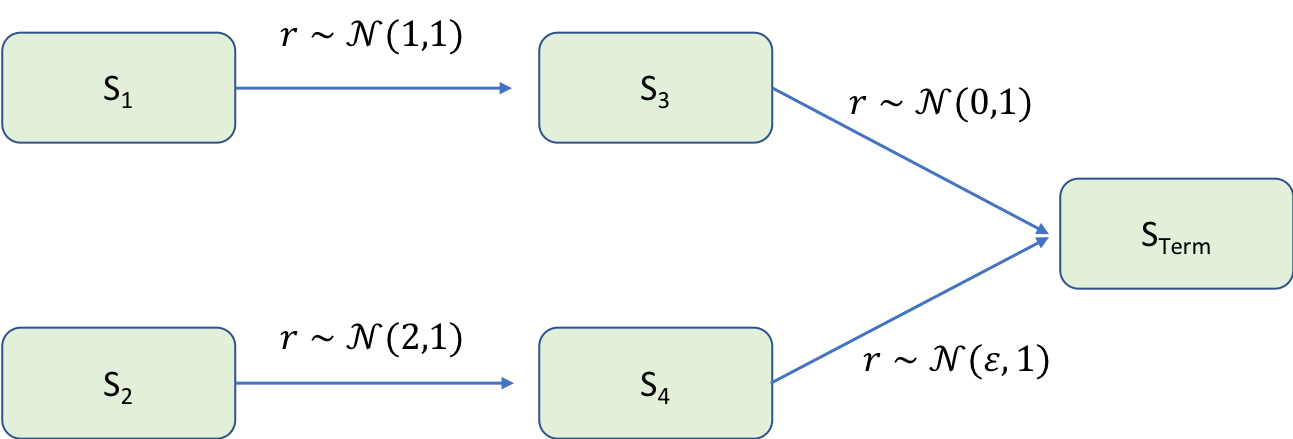
\includegraphics[width=\textwidth]{figures/td_vs_mc_FA.png}
    \caption{Example: MC vs. TD with function approximation.}
    \label{fig:td_vs_mc_FA}
\end{figure}

Consider the MDP in Figure \ref{fig:td_vs_mc_FA}, where $\state_{Term}$ is a terminal state, and rewards are normally distributed, as shown. There are no actions, and therefore for any $\policy$, $\Value^{\policy}(\state_1) = 1$, $\Value^{\policy}(\state_2) = 2+\varepsilon$, $\Value^{\policy}(\state_3) = 0$, and $\Value^{\policy}(\state_4) = \varepsilon$. We will particularly be interested in estimating $\Value^{\policy}(\state_1)$ and $\Value^{\policy}(\state_2)$.

Consider the case of no function approximation. Assume that we have sampled $N$ trajectories, where half start from $\state_1$, and the other half from $\state_2$. In this case, the MC estimates for $\widehat{\Value}^{\policy}(\state_1)$ and $\widehat{\Value}^{\policy}(\state_2)$ will each be based on $N/2$ samples, and their variance will therefore be $2 / ({N}/{2}) = 4/{N}$.

Let us recall the bootstrapping approach. We have that $\Value^{\policy}(\state_1) = \mathbb{E}\left[ \reward(\state_1)\right] + \Value^{\policy}(\state_3)$, and similarly, $\Value^{\policy}(\state_2) = \mathbb{E}\left[ \reward(\state_2)\right] + \Value^{\policy}(\state_4)$. Therefore, we can use the samples to first estimate $\widehat{\Value}^{\policy}(\state_3)$ and $\widehat{\Value}^{\policy}(\state_4)$, and then plug in to estimate $\widehat{\Value}^{\policy}(\state_1)$ and $\widehat{\Value}^{\policy}(\state_2)$.

Now, for small $\varepsilon$, we understand that the values $\Value^{\policy}(\state_3)$ and $\Value^{\policy}(\state_4)$ should be similar. One way to take this into account is to use function approximation that approximates $\Value^{\policy}(\state_3)$ and $\Value^{\policy}(\state_4)$ as \textit{the same} value, $\widehat{\Value}_{3/4}$. In this approximation we effectively use the full $N$ samples to estimate $\widehat{\Value}_{3/4}$, resulting in variance $1/{N}$. We can now use bootstrapping to estimate $\widehat{\Value}^{\policy}(\state_1)$ and $\widehat{\Value}^{\policy}(\state_2)$, which will result in variance $1 / {N}+ 1 / ({N}/{2}) = 3/{N}$, smaller than the MC estimate!

However, note that for $\varepsilon \neq 0$, the bootstrapping solution will also be biased: taking $N\to \infty$ we see that $\widehat{\Value}_{3/4}$ will converge to $\varepsilon/2$, and therefore $\widehat{\Value}^{\policy}(\state_1)$ and $\widehat{\Value}^{\policy}(\state_2)$ will converge to $1+\varepsilon/2$ and $2+\varepsilon/2$, respectively.

Thus, we see that bootstrapping, when combined with function approximation, allowed us to reduce variance by exploiting the similarity between values of different states, but at the cost of a possible bias in the expected solution. As it turns out, this phenomenon is not limited to the example above, but can be shown to hold more generally~\cite{kearns2000bias}. \AT{I don't know of a general result about bias/variance that is simple enough to state in the book. Any ideas?}

In the following, we shall develop a rigorous formulation of bootstrapping with function approximation, and use it to suggest several approximation algorithms. We will also bound the bias incurred by this approach.

\subsection{Approximate Policy Evaluation: the Projected Bellman Equation}

% A key step in approximate policy iteration here is the policy evaluation: given $\policy$ we would like to approximate $\Value^\policy$. There are two main methods for approximate policy evaluation:
% \begin{enumerate}
% \item Direct approach: Evaluate $\Value^\policy(s)$ only for several states (e.g. by simulation) and interpolate, e.g., using least squares regression: $\FtrMtx \weights = \Pi \Value^\policy$. This method is simple, however, it has several drawbacks. The first is that value estimates typically have a large variance, as they accumulate rewards from multiple states in the future. The second is that we need to wait for full simulations to complete before updating the value estimate. Practically, this can take too long in some problems. 
% \item 
Recalling the relation between TD methods and the Bellman equation, we shall start our investigation from a fundamental equation that takes function approximation into account -- the projected Bellman equation (PBE). We will use the PBE to define a particular approximation of the value function, and study its properties. We will later develop algorithms that estimate this approximation using sampling.

We consider a linear function approximation, and let $\FtrMtx \in \mathbb{R}^{|\States|\times \nftrs}$ denote a matrix in which each row $\state$ is $\ftrs(\state)$, where without loss of generality we assume that the states are ordered as $1,2,\dots, |\States|$. 
Let $\ftrspace = \left\{ \FtrMtx \weights: \weights \in \mathbb{R}^{\nftrs} \right\}$ denote the linear subspace spanned by $\FtrMtx$.
Recall that $\Value^\policy(s)\in\mathbb{R}^{|\States|}$ satisfies the Bellman equation: $\Value^\policy = \operator^\policy \Value^\policy$. However, $\Value^\policy$ does not necessarily belong to $\ftrspace$, as we may not be able to accurately represent the true value function as a linear combination of our features. 

To write a `Bellman-like' equation that involves our function approximation, we proceed by projecting the Bellman operator $\operator^\policy$ onto $\ftrspace$, resulting in the PBE:
\begin{equation}\label{eq:PBE}
    \FtrMtx \weights = \Project_{\xi} \operator^\policy \{\FtrMtx \weights\},
\end{equation}
where $\Project_{\xi}$ is the projection operator onto $\ftrspace$ under some $\xi$-weighted Euclidean norm.

Let us try to intuitively interpret the PBE. We are looking for an approximate value function $\FtrMtx \weights \in \mathbb{R}^{|\States|}$, which by definition is within our linear approximation space, such that after we apply to it $\operator^\policy$, and project the result (which does not necessarily belong to $\ftrspace$ anymore) back to $\ftrspace$, we obtain the same approximate value. Since the true value is a fixed point of $\operator^\policy$, we have reason to believe that a fixed point of $\Project_{\xi}\operator^\policy$ may provide a reasonable approximation. In the following, we shall investigate this hypothesis, and build on Eq.~\eqref{eq:PBE} to develop various learning algorithms. We remark that the PBE is not the only way of defining an approximate value function, and other approaches have been proposed in the literature. However, the PBE is the basis for the most popular RL algorithms today.
    % \begin{equation*}
    %     \weights_k= \underset{\weights}{\operatorname{argmin}} \{||\FtrMtx \weights - T^{\policy_k}\FtrMtx \weights_k||_\xi^2\}.
    % \end{equation*}
% Includes:
% \begin{itemize}
% \item Temporal differences - TD(0): online solution of the PBE.
% % $\FtrMtx \weights = \Pi \operator^\policy \{\FtrMtx \weights\}$, where $\Pi$ is the projection operator onto $\mathcal{S}$ under some norm.\\
% \item Least-squares policy evaluation - LSPE(0): simulation-based form
% \begin{align*}\FtrMtx \weights_{k+1} = \Pi \operator^\policy \{\FtrMtx \weights_k\} + \mathrm{noise}.\end{align*} 
% \item Least-squares temporal differences - LSTD(0): batch solution of the PBE.
% \end{itemize}
% \end{enumerate}

% We now discuss the indirect approach to policy evaluation.

% Define the weighted Euclidean inner product:
% $$\langle V_1,V_2\rangle_\xi = {\sum_{i=1}^n \xi_i V_1(i)V_2(i)}, \ \ \xi_i\ge0,$$
% and the induced weighted Euclidean norm:
% $$||V||_\xi = \sqrt{\langle V,V\rangle_\xi} = \sqrt{\sum_{i=1}^n \xi_i V(i)^2}, \ \ \xi_i\ge0,$$
% and let $\Project_\xi$ be the operator of projection onto $\mathcal{S}$ w.r.t. this norm:
% \begin{align*}\Project_\xi V &=\underset{V' \in \mathcal{S}}{\operatorname{argmin}} \ ||V'-V||_\xi =\\
% &= \FtrMtx \weights \ \ \ \mathrm{s.t.} \ \ \weights = \underset{\weights' \in \mathbb{R}^k}{\operatorname{argmin}} \ ||\FtrMtx \weights' - V||_\xi.\end{align*}

% We want to solve the projected Bellman equation (PBE):
% \begin{equation}\label{eq:PBE}
% \FtrMtx \weights^*  = \Project_\xi \operator^\policy \FtrMtx \weights^*.
% \end{equation}
% The main reason to consider the approximation in \eqref{eq:PBE} is that, as we shall see, it will allow us to derive efficient sampling based algorithms with provable error guarantees.

\subsubsection{Existence, Uniqueness and Error Bound on PBE Solution}
We are interested in the following questions:
\begin{enumerate}
\item Does the PBE \eqref{eq:PBE} have a solution?
\item When is $\Project_\xi \operator^\policy$ a contraction, and what is its fixed point?
\item If $\Project_\xi \operator^\policy$ has a fixed point $\FtrMtx\weights^*$, how far is it from the best approximation possible, namely, $\Project_\xi  \Value^\policy$?
\end{enumerate}
Answering the first two points will characterize the approximate solution we seek. The third point above relates to the bias of the bootstrapping approach, as described in the example in Section \ref{ssec:APE_bootstrapping}. 

Let us assume the following:
\begin{assumption}\label{ass:recurrent}The Markov chain corresponding to $\policy$ has a single recurrent class and no transient states. We further let
$$\xi_j = \lim_{N\rightarrow \infty} \frac{1}{N} \sum_{\ttime=1}^N P(\state_\ttime=j|\state_0=\state)>0,$$
which is the probability of being in state $j$ when the process reaches its steady state, given any arbitrary $\state_0=\state$.
\end{assumption}
We have the following result:
\begin{proposition}\label{prop:PBE_contraction} Under Assumption \ref{ass:recurrent} we have that
\begin{enumerate}
\item $\Project_\xi \operator^\policy$ is a contraction operator with modulus $\gamma$ w.r.t. $||\cdot||_\xi$.
\item The unique fixed point $\FtrMtx \weights^*$ of $\Project_\xi \operator^\policy$ satisfies,
\begin{equation}\label{eq:bias_bound_1}
    ||\Value^\policy - \FtrMtx \weights^*||_\xi \le \frac{1}{1-\gamma}||\Value^\policy-\Project_\xi\Value^\policy||_\xi,
\end{equation}
and
\begin{equation}\label{eq:bias_bound_2}
||\Value^\policy - \FtrMtx \weights^*||_\xi^2 \le \frac{1}{1-\gamma^2}||\Value^\policy-\Project_\xi \Value^\policy||_\xi^2.
\end{equation}
\end{enumerate}
\end{proposition}

We remark that the bound in \eqref{eq:bias_bound_2} is stronger than the bound in  \eqref{eq:bias_bound_1} (show this!). We nevertheless include the bound \eqref{eq:bias_bound_1} for didactic purpose, as it's proof is slightly different.
Proposition \ref{prop:PBE_contraction} shows that for the particular projection defined by weighting the Euclidean norm according to the stationary distribution of the Markov chain, we can both guarantee a solution to the PBE, and bound its bias with respect to the best solution possible under this weighting, $\Project_\xi \Value^\policy$. Fortunately, we shall later see that this specific weighting is suitable for developing on-policy learning algorithms. However, the reader should note that for a different $\xi$, the conclusions of Proposition \ref{prop:PBE_contraction} do not necessarily hold.

\begin{proof}
We begin by showing the contraction property. We use two lemmas.
\begin{lemma}\label{lem:P_non_expansion} If $P^\policy$ is the transition matrix induced by $\policy$, then
$$\forall z \ \ ||P^\policy z||_\xi \le ||z||_\xi.$$
\end{lemma}
\begin{proof}
Let $p_{ij}$ be the components of $P^\policy$. For all $z \in \mathbb{R}^{|\States|}$:
$$||P^\policy z||_\xi^2 = \sum_i \xi_i\left(\sum_j p_{ij}z_j\right)^2 \underbrace{\leq}_{\textrm{Jensen}} \sum_i \xi_i \sum_j p_{ij} z_j^2 =  \sum_j z_j^2 \sum_i\xi_i p_{ij} = ||z||_\xi^2,$$
where the last equality is since by definition of $\xi_i$, $\sum_i\xi_i p_{ij}  =\xi_j$, and
$\sum_{j=1}^n\xi_j z_j^2 = ||z||_\xi^2.$
\end{proof}
%\textcolor{red}{Yishay, I didn't find a proof for the lemma above in the MC or other chapters. Let me know if I missed something. Answer: Theorem 3.3 has something related, but let's keep the proof.}
\begin{lemma}\label{lem:pythagorian}
The projection $\Project_\xi$ obeys the Pythagorian theorem:
$$\forall J\in \mathbb{R}^{|\States|}, \widehat{J}\in \ftrspace: \ \ ||J-\widehat{J}||_\xi^2 = ||J-\Project_\xi J||_\xi^2 + ||\Project_\xi J - \widehat{J}||_\xi^2.$$
\end{lemma}
\begin{proof}
% Since $\Project_\xi$ is a projection with respect to a weighted Euclidean norm, it obeys the Pythagorian theorem:
%First, let's observe that the Pythagorian theorem holds for $||\cdot||_\xi$, and therefore
Observe that
$$||J-\widehat{J}||_\xi^2 = ||J-\Project_\xi J + \Project_\xi J - \widehat{J}||_\xi^2 = ||J-\Project_\xi J||_\xi^2 + ||\Project_\xi J - \widehat{J}||_\xi^2 + 2 \cdot \langle J-\Project_\xi J, \Project_\xi J - \widehat{J}\rangle_\xi.$$
We claim that $J-\Project_\xi J$ and $\Project_\xi J-\widehat{J}$ are orthogonal under $\langle\cdot,\cdot\rangle_\xi$ (this is known as the error orthogonality for weighted Euclidean-norm projections). To see this, recall that 
$$
\Project_\xi = \FtrMtx (\FtrMtx^T \Xi \FtrMtx)^{-1} \FtrMtx^T \Xi,
$$
so
$$
\Xi \Project_\xi = \Xi \FtrMtx (\FtrMtx^T \Xi \FtrMtx)^{-1} \FtrMtx^T \Xi = \Project_\xi^T \Xi.
$$
Now, 
\begin{equation*}
    \begin{split}
        \langle J-\Project_\xi J, \Project_\xi J - \widehat{J}\rangle_\xi &= (J-\Project_\xi J)^T \Xi (\Project_\xi J - \widehat{J}) \\
        &= J^T \Xi \Project_\xi J - J^T \Xi \widehat{J} - J^T \Project_\xi^T \Xi \Project_\xi J + J^T \Project_\xi^T \Xi \widehat{J} \\
        &= J^T \Xi \Project_\xi J - J^T \Xi \widehat{J} - J^T \Xi \Project_\xi \Project_\xi J + J^T \Xi\Project_\xi \widehat{J} \\
        &= J^T \Xi \Project_\xi J - J^T \Xi \Project_\xi J - J^T \Xi \widehat{J} + J^T \widehat{J} = 0,
    \end{split}
\end{equation*}
where in the penultimate equality we used that fact that $\Project_\xi \widehat{J} = \widehat{J}$, as $\widehat{J}\in \ftrspace$, and that $\Project_\xi \Project_\xi = \Project_\xi$, as projecting a vector that is already in $\ftrspace$ effects no change to the vector.
\end{proof}

We now claim that that $\Project_\xi$ is non-expansive.
\begin{lemma}
We have that $\forall {J}_1,{J}_2\in \mathbb{R}^{|\States|}, ||\Project_\xi {J}_1 - \Project_\xi {J}_2||_\xi \le ||{J}_1-{J}_2||_\xi$.
\end{lemma}

\begin{proof}
We have
$$||\Project_\xi {J}_1 - \Project_\xi {J}_2||_\xi^2 = ||\Project_\xi({J}_1-{J}_2)||_\xi^2 \le ||\Project_\xi({J}_1-{J}_2)||_\xi^2 + ||(I-\Project_\xi)({J}_1-{J}_2)||_\xi^2 = ||{J}_1-{J}_2||_\xi^2,$$
where the first inequality is by linearity of $\Project_\xi$, and the last equality is by the Pythagorean theorem of Lemma \ref{lem:pythagorian}, where we set $J={J}_1-{J}_2$ and $\widehat{J} = 0$.
\end{proof}

In order to prove the contraction $\forall {J}_1,{J}_2\in \mathbb{R}^{|\States|}$:
\begin{equation*}
\begin{split}
||\Project_\xi \operator^\policy {J}_1 - \Project_\xi \operator^\policy {J}_2||_\xi &\overset{\Project_\xi \textrm{ non-expansive}}{\le} ||\operator^\policy {J}_1 - \operator^\policy {J}_2||_\xi\\
&\overset{\textrm{definition of } \operator^\policy}{=} \gamma||P^\policy({J}_1-{J}_2)||_\xi \overset{\textrm{Lemma \ref{lem:P_non_expansion}}}{\le} \gamma||{J}_1-{J}_2||_\xi ,
\end{split}
\end{equation*}
and therefore $\Project_\xi \operator^\policy$ is a contraction operator.

We now prove the error bound in \eqref{eq:bias_bound_1}.
\begin{equation*}
\begin{split}
  ||\Value^\policy - \FtrMtx \weights^*||_\xi  &\leq ||\Value^\policy
-\Project_\xi \Value^\policy||_\xi + ||\Project_\xi \Value^\policy -\FtrMtx \weights^*||_\xi  \\
    &= ||\Value^\policy -\Project_\xi \Value^\policy||_\xi + ||\Project_\xi \operator^\policy \Value^\policy -\Project_\xi \operator^\policy\FtrMtx \weights^*||_\xi \\
&\leq ||\Value^\policy -\Project_\xi \Value^\policy||_\xi + \gamma||\Value^\policy-\FtrMtx \weights^*||_\xi,
\end{split}
\end{equation*}
where the first inequality is by the triangle inequality, the second equality is since $\Value^\policy$ is $\operator^\policy$'s fixed point, and $\FtrMtx \weights^*$ is $\Project_\xi \operator^\policy$'s fixed point, and the second inequality is by the contraction of $\Project_\xi \operator^\policy$. Rearranging gives \eqref{eq:bias_bound_1}.

We proceed to prove the error bound \eqref{eq:bias_bound_2}.
\begin{equation}
\begin{split}
  ||\Value^\policy - \FtrMtx \weights^*||_\xi^2  &= ||\Value^\policy
-\Project_\xi \Value^\policy||_\xi^2 + ||\Project_\xi \Value^\policy -\FtrMtx \weights^*||_\xi^2  \\
    &= ||\Value^\policy -\Project_\xi \Value^\policy||_\xi^2 + ||\Project_\xi \operator^\policy \Value^\policy -\Project_\xi \operator^\policy\FtrMtx \weights^*||_\xi^2 \\
&\leq ||\Value^\policy -\Project_\xi \Value^\policy||_\xi^2 + \gamma^2||\Value^\policy-\FtrMtx \weights^*||_\xi^2,
\end{split}
\end{equation}
where the first equality is by the Pythagorean theorem, and the remainder follows similarly to the proof of \eqref{eq:bias_bound_1} above.
% the second equality is since $\Value^\policy$ is $\operator^\policy$'s fixed point, and $\FtrMtx \weights^*$ is $\Project_\xi \operator^\policy$'s fixed point, and the inequality is by the contraction of $\Project_\xi \operator^\policy$.

% Therefore
% $$||\Value^\policy - \FtrMtx \weights^*||_\xi^2 \le \frac{1}{1-\gamma^2}||\Value^\policy-\Project_\xi \Value^\policy||_\xi^2.$$
\end{proof}

% \begin{remark}
% A weaker error bound of $||\Value^\policy - \FtrMtx \weights^*||_\xi \le \frac{1}{1-\gamma}||\Value^\policy-\Project_\xi
% \Value^\policy||_\xi$ may be obtained by the following argument:
% \begin{equation}
% \begin{split}
%   ||\Value^\policy - \FtrMtx \weights^*||_\xi  &\leq ||\Value^\policy
% -\Project_\xi \Value^\policy||_\xi + ||\Project_\xi \Value^\policy -\FtrMtx \weights^*||_\xi  \\
%     &= ||\Value^\policy -\Project_\xi \Value^\policy||_\xi + ||\Project_\xi \operator^\policy \Value^\policy -\Project_\xi \operator^\policy\FtrMtx \weights^*||_\xi \\
% &\leq ||\Value^\policy -\Project_\xi \Value^\policy||_\xi + \gamma||\Value^\policy-\FtrMtx \weights^*||_\xi,
% \end{split}
% \end{equation}
% where the first inequality is by the triangle inequality.
% \end{remark}
% \begin{remark}
% The error bounds in this section are in the $\| \cdot \|_\xi$ norm, while the approximate policy iteration error bounds of Theorem \ref{thm:API} are in the $\| \cdot \|_\infty$ norm. In general, for large or continuous state spaces, an $\| \cdot \|_\xi$ norm error bound does not provide a strong guarantee on the error in the $\| \cdot \|_\infty$ norm, and the results of Theorem \ref{thm:API} therefore do not apply. A result similar to that of Theorem \ref{thm:API} may be shown to hold in the $\| \cdot \|_\xi$ norm, however this is much more complicated, and beyond the scope of this course.
% \end{remark}
% \begin{remark}
% At this point, the reader should wonder why the PBE solution is sought instead of $\Project_\xi \Value^\policy$. In fact, an algorithm for estimating $\Project_\xi \Value^\policy$ can easily be derived using regression. For example, consider an algorithm that samples states $s_1,\dots,s_N \sim \xi$, and from each state $s_i$ runs a trajectory in the MDP following policy $\policy$. Let $y_i$ denote the discounted return in that trajectory. Then, a least squares fit:
% \begin{equation*}
%     \min_\weights \frac{1}{2}\sum_{i=1}^{N} \left(y_i - \ftrs(s_i)^\top\weights\right)^2
% \end{equation*}
% would converge to $\Project_\xi \Value^\policy$ as $N\to \infty$. However, such an algorithm would suffer a high variance, since the discounted return in the whole trajectory often has a high variance. The PBE approach typically has lower variance, since it only considers 1-step transitions instead of complete trajectories. However, it may have a \emph{bias}, as seen by the error bound in Proposition \ref{prop:PBE_contraction}. We thus have a bias-variance tradeoff between the direct and indirect approaches to policy evaluation.
% \end{remark}

\subsection{Solution Techniques for the Projected Bellman Equation}
We now move to solving the projected Bellman equation. Taking inspiration from the algorithms for linear least squares described above, we will seek sampling-based approximations to the solution of the PBE.

Using the explicit formulation of the projection $\Project_\xi$, we see that the PBE solution is some $\widehat{\Value} = \FtrMtx \weights^*$ where $\weights^*$ solves
$$\weights^* = \underset{{\weights \in \mathbb{R}^\nftrs}}{\operatorname{argmin}} \ ||\FtrMtx \weights - (R^\policy+\gamma P^\policy\FtrMtx \weights^*)||_\xi^2.$$
Setting the gradient to $0$, we get
$$\FtrMtx^T \Xi (\FtrMtx \weights^* - (R^\policy+\gamma P^\policy \FtrMtx \weights^*)) = 0.$$
% where $\Xi = \textrm{diag} \ (\xi_1,...,\xi_n)$.\\
% This is in fact the orthogonality condition from random signals.\\
Equivalently we can write
$$A \weights^* = b,$$
where
\begin{equation}\label{eq:A_b_TD}
A = \FtrMtx^T \Xi(I-\gamma P^\policy) \FtrMtx, \ \ b = \FtrMtx^T\Xi R^\policy.
\end{equation}

\paragraph{Solution approaches:}
\begin{enumerate}
\item \textbf{Matrix inversion (LSTD)}: $$\weights^* = A^{-1}b$$
In order to evaluate $A,b$, calculate a simulation-based approximation $\widehat{A}_k,\hat{b}_k \rightarrow A,b$ by the law of large numbers, and then use $\widehat{\weights}_k = \widehat{A}_k^{-1} \widehat{b}_k$. This approach is termed the Least Squares Temporal Difference algorithm (LSTD). Note that the simulation must use the policy $\policy$, such that (after some mixing time) the states are samples from the stationary distribution $\xi$.\\
Recall that
$$b = \FtrMtx^T \Xi R^\policy = \sum_{s=1}^{|\States|} \xi(s)  {\ftrs}(s) R^\policy(s).$$
So the following estimate converges to $b$:
\begin{align*}
\widehat{b}_N &= \frac{1}{N} \sum_{t=1}^N  {\ftrs}(\state_\ttime) r(\state_\ttime,\policy(\state_\ttime)) = \\
&= \frac{1}{N}\sum_{t=1}^N\sum_{s=1}^{|\States|} {\bf1}(\state_\ttime=s) {\ftrs}(s) R^\policy(s) =\\
&= \sum_{s=1}^{|\States|} {\ftrs}(s) R^\policy(s) \frac{1}{N}\sum_{t=1}^N {\bf1}(\state_\ttime=s) \underset{N\rightarrow \infty}{\longrightarrow} b .
\end{align*}
Similarly,
\begin{align*}
\widehat{A}_N &= \frac{1}{N} \sum_{t=1}^N  {\ftrs}(\state_\ttime)(I-\gamma P^\policy) {\ftrs}^T(\state_\ttime) \approx \\
&\frac{1}{N} \sum_{t=1}^N {\ftrs}(\state_\ttime)( {\ftrs}^T(\state_\ttime)-\gamma {\ftrs}^T(s_{t+1}))  \underset{N\rightarrow \infty}{\longrightarrow} A .
\end{align*}

\item \textbf{Projected Value Iteration:}
Consider the iterative solution,
$$\FtrMtx \weights_{n+1} = \Project_\xi \operator^\policy \FtrMtx \weights_n = \Project_\xi(R^\policy+\gamma P^\policy \FtrMtx \weights_n),$$
which converges to $\weights^*$ since $\Project_\xi \operator^\policy$ is a contraction operator.\\

Recalling that $\Project_\xi$ relates to a least squares regression problem, the solution above describes a sequence of least squares regression problems. For the $(n+1)$'th regression problem, our independent variable is the state, $\state$, and the dependent variable is $\reward(\state) +\gamma \sum_{\state'}P^\policy(\state'|\state) \ftrs(\state')^T \weights_n$.

If we sample trajectories from $\policy$, after some mixing time $\ttime$, a pair of consecutive state $\state_\ttime, \state_{\ttime+1}$ are sampled from $\xi(\state)$ and $P^\policy(\state'|\state)\xi(\state)$, respectively. Therefore, we can define the samples for the least squares regression problem as $\left\{(\state_\ttime, \reward(\state_\ttime) +\gamma \ftrs(\state_{\ttime+1})^T \weights_n), \dots  (\state_{\ttime+N}, \reward(\state_{\ttime+N}) +\gamma \ftrs(\state_{\ttime+N+1})^T \weights_n)\right\}$.

% The projection step is
% $$ \weights_{n+1} = \underset{\weights}{\operatorname{argmin}}||\FtrMtx \weights - (R^\policy+\gamma P^\policy \FtrMtx \weights_n)||_\xi^2.$$
% Setting the gradient to $0$ w.r.t. $\weights$:
% $$\FtrMtx^T \Xi(\FtrMtx \weights_{n+1} - (R^\policy+\gamma P^\policy \FtrMtx \weights_n)) = 0$$
% $$\Rightarrow \weights_{n+1} = \weights_n - (\FtrMtx^T\Xi\FtrMtx)^{-1}(A \weights_n-b).$$
% So we can approximate
% $$\weights_{n+1} = \weights_n - G_n(A_n \weights_n -b_n),$$
% where
% $$G_n^{-1} \approx \frac{1}{n+1} \sum_{t=0}^n  {\ftrs}(\state_\ttime) {\ftrs}(\state_\ttime)^T \Rightarrow G_n \approx (\FtrMtx^T \Xi \FtrMtx)^{-1}.$$
% We observe that $A_n,b_n,G_n$ can also be computed via the SA algorithm.

\begin{remark}
Projected value iteration can be used with more general regression algorithm. Let $\Project_{gen}$ denote a general regression algorithm, such as a non-linear least squares fit, or even a non-parametric regression such as K-nearest neighbors. We can consider the iterative algorithm:
$$\widehat{\Value}(\weights_{n+1}) = \Project_{gen} \operator^\policy \widehat{\Value}(\weights_{n}).$$
To realize this algorithm, we use the same samples as above, and only replace the regression algorithm. Note that convergence in this case is not guaranteed, as in general, $\Project_{gen} \operator^\policy$ is not necessarily a contraction in any norm.
\end{remark}

\item \textbf{Stochastic Approximation -- TD(0):} Consider the function-approximation variant of the TD(0) algorithm (cf. Section \ref{sec:TD})
\begin{equation}\label{eq:TD_func_approx}
    \weights_{\ttime+1} = \weights_\ttime + \alpha_\ttime \underbrace{( \reward(\state_\ttime,\policy(\state_\ttime)) +\discount {\ftrs}(\state_{\ttime+1})^\top \weights_\ttime - {\ftrs}(\state_{\ttime})^\top \weights_\ttime)}_{\textrm{temporal difference}} \ftrs(\state_{\ttime}),
\end{equation}
where the temporal difference term is the approximation (w.r.t. the weights at time $\ttime$) of $\reward(\state_\ttime,\policy(s_\ttime)) +\discount \Value(\state_{\ttime+1}) - \Value(s_\ttime)$.
\\
This algorithm can be written as a stochastic approximation:
\begin{equation*}
    \weights_{\ttime+1} = \weights_\ttime + \alpha_\ttime ( b -  A \weights_\ttime + \omega_\ttime ),
\end{equation*}
where $\omega_\ttime$ is a noise term, and the corresponding ODE is $\dot{\weights} = b -  A \weights_\ttime$, with a unique stable fixed point at $\weights^* = A^{-1}b$. 

We next prove convergence of TD(0). For simplicity, we will consider a somewhat synthetic version of TD(0) where at each iteration $\ttime$, the state $\state_\ttime$ is drawn i.i.d. from the stationary distribution $\xi(\state)$, and the next state $\state_{\ttime+1}$ in the update rule is drawn from $P^\policy(\state'|\state = \state_\ttime)$, respectively. This will allow us to claim that the noise term satisfies $\E[\omega_\ttime|h_{\ttime-1}]=0$. 

\begin{remark}
A similar convergence result holds for the standard TD(0) of Eq.~\ref{eq:TD_func_approx}, using a more sophisticated proof technique that accounts for noise that is correlated (depends on the state). The main idea is to show that since the Markov chain mixes quickly, the \textit{average} noise is still close to zero with high probability~\cite{TsitsiklisVR97}.
\end{remark}

\begin{theorem}
    Consider the following iterative algorithm:
    \begin{equation*}\label{eq:TD_func_approx_iid}
    \weights_{\ttime+1} = \weights_\ttime + \alpha_\ttime ( \reward(\state_\ttime,\policy(\state_\ttime)) +\discount {\ftrs}(\state_{\ttime}')^\top \weights_\ttime - {\ftrs}(\state_{\ttime})^\top \weights_\ttime) \ftrs(\state_{\ttime}),
\end{equation*}
where $\state_\ttime\sim \xi(\state)$ i.i.d., and $\state_{\ttime}' \sim P^\policy(\state'|\state = \state_\ttime)$ independently of the history up to time $t$.
\end{theorem}

\end{enumerate}
% \begin{remark}
For a general (not necessarily linear) function approximation, the TD(0) algorithm takes the form:
\begin{equation*}
    \weights_{n+1} = \weights_n + \alpha_n \left( \reward(\state_n,\policy(\state_n)) + \widehat{\Value}(\state_{n+1},\weights_n) - \widehat{\Value}(\state_{n},\weights_n) \right) \nabla_{\weights} \widehat{\Value}(\state_n,\weights).
\end{equation*}
It can be derived as a stochastic gradient descent algorithm for the loss function
\begin{equation*}
    Loss(\weights) = ||\widehat{\Value}(\state,\weights) - \Value^\policy(\state)||_\xi,
\end{equation*}
and replacing the unknown $\Value^\policy(\state)$ with a Bellman-type estimator $\reward(\state,\policy(\state))+f(\state',\weights)$.
% \end{remark}
%\end{document}
%~

\section{Approximate Policy Optimization}

So far we have developed various algorithms for approximating the value of a fixed policy $\policy$. Our main interest, however, is finding a \textit{good} policy. Similarly to RL without function approximation, we will consider two different approaches, based on either policy iteration or value iteration.

\subsection{Approximate Policy Iteration}

\paragraph{The algorithm:} iterate between projection of $\Value^{\policy_k}$ onto $\ftrspace$ and policy improvement via a greedy policy update w.r.t. the projected $\Value^{\policy_k}$.
%$\operator^\policy$ (recall $\operator^\policy V = R^\policy + \gamma  P\policy V$, and Bellman's operator satisfies $TV = \max_{\policy \in \Pi} \operator^\policy V$):

\vspace{20pt}
\tikzstyle{block} = [rectangle, draw,
    text width=7em, text centered, rounded corners, minimum height=4em]
\tikzstyle{line} = [draw, -latex']
\begin{tikzpicture}[node distance = 2cm, auto]
    % Place nodes
    \node [block, node distance=1.5in, text width=3em] (a) {Guess $\policy_0$};
    \node [block, node distance=2in, right of =a, text width=15em] (b) {evaluate: \\ $\widehat{\Value}_k=\FtrMtx \weights_k \approx \Value^{\policy_{k}}$ };
    \node [block, node distance=2in, right of = b, text width=5em] (c) {improve: $\policy_{k+1}$};
    % Draw edges
    \path [line] (a) -- (b);
    \path [line] (b) -- (c);
    \path [line,rounded corners] (c) |- ($(b.south east) + (0.5,-0.5)$) -| (b);
\end{tikzpicture}
\vspace{20pt}

The key question in approximate policy iteration, is how errors in the value-function approximation, and possibly also errors in the greedy policy update, affect the error in the final policy. The next result shows that if we can guarantee that the value-function approximation error is bounded at each step of the algorithm, then the error in the final policy will also be bounded. This result suggests that approximate policy iteration is a fundamentally sound idea.

\begin{theorem}\label{thm:API}
If for each iteration $k$ the policies are approximated well over $\States$:
$$\max_\state |\widehat{\Value}_k(\state)-\Value^{\policy_k}(\state)| \le \delta,$$
and policy improvement approximates well
$$ \max_\state |\operator^{\policy_{k+1}}\widehat{\Value}_k - \operator\widehat{\Value}_k| < \varepsilon,$$
Then
$$ \limsup_k \ \max_\state | \Value^{\policy_k}(\state)-\Value^*(\state)| \le \frac{\varepsilon+2\gamma\delta}{(1-\gamma)^2}.$$
\end{theorem}

\subsection{Approximate Policy Iteration Algorithms}

We next discuss several algorithms that implement approximate policy iteration.

\subsubsection{Online - SARSA}
As we have seen earlier, it is easier to define a policy improvement step using the $Q$ function. We can easily modify the TD(0) algorithm above to learn $\widehat{Q}^\policy(\state,\action) = f(\state,\action;\weights)$:
\begin{equation*}
    \weights_{n+1} = \weights_n + \alpha_n \left( r(\state_n,a_n) + f(\state_{n+1},\action_{n+1};\weights_n) - f(\state_{n},\action_{n}; \weights_n) \right) \nabla_{\weights} f(\state_n,\action_n,\weights).
\end{equation*}
The actions are typically selected according to an $\xi-$greedy or softmax rule. Thus, policy evaluation is interleaved with policy improvement.

\subsubsection{Batch - Least Squares Policy Iteration (LSPI)}
One can also derive an approximate policy iteration algorithm that works on a batch of data. Consider the linear case $\widehat{Q}^\policy(\state,\action) = \weights^T \ftrs(\state,\action)$. The idea is to use LSTD(0) to iteratively fit $\widehat{Q}^{\policy_k}$, where $\policy_k$ is the greedy policy w.r.t. $\widehat{Q}^{\policy_{k-1}}$.

\begin{align*}
\widehat{b}_n^k &= \frac{1}{n} \sum_{\ttime=1}^n  {\ftrs}(\state_\ttime, \action_\ttime) \reward(\state_\ttime,\action_\ttime) 
\end{align*}
\begin{align*}
\widehat{A}_n^k &= \frac{1}{n} \sum_{t=1}^n {\ftrs}(\state_\ttime,\action_\ttime)( {\ftrs}^T(\state_\ttime,\action_\ttime)-\gamma {\ftrs}^T(\state_{t+1},\action^*_{t+1})),
\end{align*}
\begin{align*}
\weights_k &= (\widehat{A}_n^k)^{-1} \widehat{b}_n^k.
\end{align*}
where $\action^*_{t+1} = \argmax_\action \widehat{Q}^{\policy_{k-1}}(\state_{t+1},\action) = \argmax_\action \weights_{k-1}^T\ftrs(\state_{t+1},\action)$.

\subsection{Approximate Value Iteration}
Approximate value iteration algorithms directly approximate the optimal value function (or optimal $Q$ function). Let us first consider the linear case. The idea in approximate VI is similar to the PBE, but replacing $\operator^\policy$ with $\operator^*$. That is, we seek solutions to the following projected equation:
\begin{equation*}
    \FtrMtx \weights = \Project \operator^* \{\FtrMtx \weights\},
\end{equation*}
where $\Project$ is some projection, such as the weighted least squares projection $\Project_\xi$ considered above. Recall that $\operator^*$ is a contraction in the $\|.\|_\infty$ norm. Unfortunately, $\Pi$ is not necessarily a contraction in $\|.\|_\infty$ for general function approximation, and not even for the weighted least squares projection $\Project_\xi$.\footnote{A restricted class of function approximators for which contraction does hold is called averagers, as was proposed in \cite{gordon1995stable}. The k-nearest neighbors approximation, for example, is an averager.} On the other hand, $\operator^*$ is not a contraction in the $\|.\|_\xi$ norm. Thus, we have no guarantee that the projected equation has a solution. Nevertheless, algorithms based on this approach have achieved impressive success in practice. 

% For the non-linear case, we have:
% \begin{equation*}
%     \widehat{Q}(\weights_{n+1}) = \Pi T \widehat{Q}(\weights_{n}).
% \end{equation*}

\subsubsection{Online - Q Learning}
The function approximation version of online Q-learning resembles SARSA, only with an additional maximization over the next action:
\begin{equation*}
    \weights_{n+1} = \weights_n + \alpha_n \left( \reward(\state_n,\action_n) + \max_\action \widehat{Q}(\state_{n+1},\action;\weights_n) - \widehat{Q}(\state_{n},\action_{n}; \weights_n) \right) \nabla_{\weights} \widehat{Q}(\state_n,\action_n,\weights).
\end{equation*}
The actions are typically selected according to an $\varepsilon-$greedy or softmax rule, to balance exploration and exploitation.

\subsubsection{Batch -- Fitted Q}

In this approach, we iteratively project (fit) the Q function based on the projected equation:
\begin{equation*}
    \widehat{Q}(\weights_{n+1}) = \Project \operator^* \widehat{Q}(\weights_{n}).
\end{equation*}

Assume we have a data set of samples $\{\state_i,\action_i,\state'_i,\reward_i\}$,obtained from some data collection policy. Then, the right hand side of the equation denotes a regression problem where the samples are: $\left\{(\state_i,\action_i), r_i + \gamma \max_\action \widehat{Q}(\state'_i, \action;\weights_{n})\right\}$. Thus, by solving a sequence of regression problems we approximate a solution to the projected equation.

Note that approximate VI algorithms are \emph{off-policy} algorithms. Thus, in both Q-learning and fitted-Q, the policy that explores the MDP can be arbitrary (assuming of course it explores `enough' interesting states).

\section{Off-Policy Learning with Function Approximation}
\label{sec:off_policy_FA}

We would like to see what is the effect that the samples are generated
following a different policy, namely, an off-policy setting. There
is no issue for Monte-Carlo, and the same logic would still be
valid.  For TD, we did not have any problem in the look-up model. We
would like to see what can go wrong when we have a function
approximation setting.


\begin{figure}
  % Requires \usepackage{graphicx}
  \begin{centering}
  \includegraphics[width=0.5\textwidth]{figures/L8-2states.png}\\
  \caption{Two state snippet of an MDP }\label{fig:L8-2state}
  \end{centering}
\end{figure}

Consider the following part of an MDP (see Figure
\ref{fig:L8-2state}) consists of two nodes, with a transition from
the first to the second, with reward $0$. The main issue is that the
linear approximation gives the first node a weight $\weight$ and the
second $2\weight$. Assume we start with some value $\weight_0>0$.
Each time we have an update for the two states we have
\[
\weight_{\ttime+1}=\weight_\ttime +\alpha[0+\gamma
(2\weight_\ttime)-\weight_\ttime]=[1+\alpha(2\gamma-1)]\weight_\ttime=[1+\alpha(2\gamma-1)]^\ttime\weight_1
\]
For $\gamma>0.5$ we have $\alpha(2\gamma-1)>0$, and $\weight_\ttime$
diverges.

We are implicitly assuming that the setting is off-policy, since in
an on-policy, we would continue from the second state, and
eventually lower the weight.

To have a ``complete'' example consider the three state MDP in
Figure~\ref{fig:L8-3state}. All the rewards are zero, and the main
difference is that we have a new terminating state, that we reach
with probability $p$.

\begin{figure}
  % Requires \usepackage{graphicx}
  \begin{centering}
  \includegraphics[width=0.5\textwidth]{figures/L8-3state.png}\\
  \caption{The three state MDP. All rewards are zero.}\label{fig:L8-3state}
  \end{centering}
\end{figure}




Again, assume that we start with some $\weight_0>0$ We have three
types of updates, one per possible transition. When we transition
from the initial state to the second state we have
\[
\Delta \weight= \alpha[0+\gamma
(2\weight_\ttime)-\weight_\ttime]\cdot
1=\alpha(2\gamma-1)\weight_\ttime
\]
The transition from the second state back to itself has an update,
\[
\Delta \weight= \alpha[0+\gamma
(2\weight_\ttime)-(2\weight_\ttime)]\cdot 2
=-4\alpha(1-\gamma)\weight_\ttime
\]
The transition to the terminal state we have
\[
\Delta \weight= \alpha[0+\gamma 0 -(2\weight_\ttime)]\cdot
2=-4\alpha \weight_\ttime
\]



When we use on-policy, we have all transitions. Assume that the
second transition happens $n\geq 0$ times. Then we have
\[
\frac{\weight_{\ttime+1}}{\weight_\ttime}=(1+\alpha(2\gamma-1))(1-4\alpha(1-\gamma))^n(1-4\alpha)<
1-\alpha
\]
This implies that $\weight_\ttime$ converges to zero, as desired.

Now consider an off-policy that truncates the episodes after $n$
transitions of the second state, where $n\ll 1/p$, and in addition
$\gamma> 1-1/(40n)$. This implies that in most updates we do not
reach the terminal state and we have
\[
\frac{\weight_{\ttime+1}}{\weight_\ttime}=(1+\alpha(2\gamma-1))(1-4\alpha(1-\gamma))^n>1
\]
and therefore, for the some setting of $n$ we have that the weight
$\weight_\ttime$ diverges.

We might hope that the divergence is due to the online nature of the
TD updates. We can consider an algorithm that in each iteration
minimizes the square error. Namely,
\[
\weight_{\ttime+1}=\arg\min_\weight\sum_s
[\widehat{\Value}(\state_\ttime;\weight)-E^\policy[\reward_\ttime+\gamma\widehat{\Value}(\state_{\ttime+1};\weight_\ttime)]]^2
\]

For the MDP example of Figure~\ref{fig:L8-3state} we have that:
\begin{align*}
 \weight_{\ttime+1} &= \arg\min_\weight (\weight-\gamma(2\weight_\ttime))^2+(2\weight-(1-p)\gamma(2\weight_\ttime))^2
\end{align*}
Solving for $\weight_{\ttime+1}$ we have
\begin{align*}
0&=  2(\weight_{\ttime+1}-\gamma(2\weight_\ttime))+4(2\weight_{\ttime+1}-(1-p)\gamma(2\weight_\ttime)\\
  10 \weight_{\ttime+1}&=4\gamma \weight_\ttime + 8\gamma(1-p)\weight_\ttime\\
  \weight_{\ttime+1}&=\frac{6-4p}{5}\gamma \weight_\ttime
\end{align*}
So for $\gamma(6-4p)>5$ we have divergence. (Recall that
$\gamma\approx 1-\varepsilon$ and $p\approx \varepsilon$ is a very
important setting.)

Note that if we have taken in to account the influence of
$\weight_{\ttime+1}$ on $\Value$ and use
$\widehat{\Value}(\state_{\ttime+1};\weight_{\ttime+1})$ instead of
$\widehat{\Value}(\state_{\ttime+1};\weight_\ttime)$, this specific
problem would have disappeared, since $\weight_{\ttime+1}=0$ would
be the minimizer.

\subsubsection{Summary of convergence results} Here is a summary of the known convergence and divergence results in
the literature:
\begin{center}
  \begin{tabular}{ | l | c | c|c|c| }
    \hline
    & algorithm & look-up table&linear function&non-linear\\ \hline
    on-policy & MC & + & + & + \\ \hline
    on-policy & $TD(0),TD(\lambda)$ & + & + & -\\ \hline
 %   on-policy & $TD(\lambda)$ & + & + & - \\ \hline
    off-policy & MC & + & + & + \\ \hline
    off-policy & $TD(0),TD(\lambda)$ & + & - & -\\ \hline
 %   off-policy & $TD(\lambda)$ & + & - & - \\ \hline
  \end{tabular}
\end{center}

The results for the look-up table where derived in Chapter
\ref{chapter:learning-model-free}.
%
The fact that Monte-Carlo methods converge is due to the fact that
they are running an SGD algorithm. For linear functions with convex
loss they will converge to the global optimum and for non-linear
functions (for example, neural networks) they will converge to a
local optima. The convergence to the TD appear in Chapter
\ref{sec:FA-Advanced}. The divergence of TD with linear functions in
an off-policy setting appear in Chapter \ref{sec:TD-FA}. The TD
divergence in the non-linear online setting appears in
\cite{TsitsiklisVR97}.
